\chapter{Background: Sequence Modeling}\label{ch:ch3}
In the following chapter, we provide the background and context behind the choice of our model. Recurrent Neural Networks currently provide the foundation for state-of-the-art EMP models. Recent developments in neural sequence modeling move entirely away from RNNs and toward a new family of ANN architectures, the Transformer. Because Transformers have not seen application in EMP generation models, they are the focus of our work. 

\section{Sequential Data}\label{sec:sequential-data}
The modeling of sequence data is a fundamental aspect of modern machine learning. Sequence data consists of individual data points with a relationship to each other according to some specific order and position in time. A simple example of sequential data is the weather, which follows predictable patterns according to the time of year. Although it is difficult to predict precise weather patterns using the year alone, we can easily forecast general weather patterns (temperatures will always be warmer in the summer than in the winter). 

Musical data is also fundamentally sequential\cite{widmer2016getting} given that we experience music as events that happen in time, and the relationship of such events according to their position in time is paramount to the phenomena of musical experience. Language and speech exhibit this same property, and the research in natural language processing drives much of the research advance in neural sequential data modeling. 

Sequence data modeling is typically categorized into several different tasks. Perhaps the most common task is sequence classification, which seeks to assign some sequence of data points to a particular class of data. When using real-valued features, input data is defined as a sequence of data points $X = \{x_1, x_2, x_3, ..., x_n\}$, where each data point is an $m$-dimensional vector $x_i \in \mathbb{R}^m$. The output data is a single value $y \in L$ where $L$ is a set of class labels. A sequence classification model $C: \mathbb{R}^{n \times m} \rightarrow L$ will then map from an input sequence $X$ to a class label $y$. Email spam detection and genre classification are common use cases of sequence classification models in NLP and MIR, respectively. 

% seq for seq2seq
\newcommand{\seq}{\emph{seq2seq}}

EMP generation is a more complicated process. It involves mapping an input sequence (score) to another output sequence (performance). We call such a task a sequence-to-sequence (\seq{}) model. In this case our input data $X$ is the same, but our output data is also defined as a sequence of vectors $Y = \{y_1, y_2, y_3, ..., y_{\hat{n}}\}$, where $y_i \in \mathbb{R}^{\hat{m}}$. We can then define a \seq{} model as $S: \mathbb{R}^{n \times m} \rightarrow \mathbb{R}^{\hat{n} \times \hat{m}}$ which will produce an output sequence $Y$ given the input sequence $X$. In EMP generation, $m$ is the number of score features, $n$ is the number of input score notes, $\hat{m}$ is the number of performance features, and $\hat{n}$ the number of output performance notes. 

\section{Case Study: Neural Machine Translation}
RNNs and their common adaptations as an LSTM have historically been the default modeling choices for sequential data Deep Learning\footnote{For brevities sake, we do not provide the detailed mathematical definition for RNNs here and refer to the reader to~\citet{goodfellow2016deep}}. However, in recent years the Transformer~\cite{vaswani2017attention} architecture model has outperformed RNNs in many tasks and is becoming the de-facto standard for sequential data modeling in modern Machine Learning~\cite{devlin2018bert, brown2020language}. To provide context for the Transformer's origin, we will outline the historical progress of an NLP task known as neural machine translation (NMT). 

Machine translation (MT) is the task of computationally translating one natural language to another\footnote{\href{https://translate.google.com/}{Google Translate} is one successful commercial application.}. Traditional MT systems relied on complicated rule sets and decoding algorithms stitched together to create a statistical model known as a statistical machine translation (SMT) system. Rather than an amalgamation of several different systems developed independently, NMT systems are trained end-to-end with a single ANN architecture and significantly reduce the complexity of building MT models. NMTs are \seq{} models and typically operate by translating a single sentence at a time.

% ed for encoder decoder
\newcommand{\ed}{\emph{encoder-decoder}}
One of the challenges in building an MT systems is that the source and target sentences are often not the same lengths - $n \neq \hat{n}$ in our definition of \seq{} models given in section \ref{sec:sequential-data}. NMT translation systems use what is known as an \ed{} architecture to address the variable-length input and output sequences. From a probabilistic perspective, the job of the \ed{} architecture is to model the conditional probability distribution of a variable-length output sentence $Y$ given a variable-length input sequence $X$, as
\begin{align*}
P(y_1, y_2, ... y_n | x_1, x_2, ..., x_l). 
\end{align*}
In the \ed{} architecture, calculation of the distribution is decomposed into two separate models. The encoder's job is to read in the source sequence and find a good representation, or encoding, of that sequence. In the original formulation of the \ed{} NMT architecture,~\citet{cho2014learning} present this encoding in the form of a fixed size vector $c$. The decoder is an autoregressive language model%
\footnote{Autoregressive models are sequence-based models that take as input the model's output at previous time steps. Language models are instances of autoregressive models that are capable of generating novel texts of varying lengths. Language models can generate novel text from scratch, although they are often \href{https://transformer.huggingface.co/doc/distil-gpt2}{prompted with existing text to write in a particular style or on a certain subject}.}, and uses $c$ as a condition to \emph{generate} the new sentence in the target language. Using this decomposition, we can view the decoder as calculating the probability of the next word in the sentence given all of the previous words and the hidden encoding vector~\cite{bahdanau2014neural}. This probability distribution is given as
\begin{align*}
P(Y) = \prod_{\hat{n}=1}^{n}P(y_i \vert y_1, y_2, ..., y_{i-1}, c)    
\end{align*}


\newcommand{\at}[1]{\emph{#1}}

The RNN-based \ed{} model of~\citet{cho2014learning} achieved state-of-the-art in MT, improving upon the results of SMT systems. However, there is an inherent limit imposed on the system for long sentences.~\citet{cho2014learning} show that the performance of a basic \ed{} model deteriorates rapidly as the length of an input sentence increases. To account for this,~\citet{bahdanau2014neural} present the foundations for what has become known as the \at{attention} mechanism. Instead of using a fixed-sized vector encoding, \at{attention} allows the decoder model to search for a set of positions in the source sentence where the most relevant information is concentrated and uses this information as it generates text in the target language. In simpler terms, the decoder ``pays attention'' to the source sentence's most relevant words to find the right translation of every word at each time step. 

Rather than use a fixed-length vector at every time step, the decoder is modeled as follows 
\begin{align*}
P(y_t \vert y_1, y_2, ..., y_{t-1}, X) = g(y_{i-1}, s_i, c_i)    
\end{align*}
where $g$ is some non-linear potentially multi-layered function that outputs the probability of $y_{t}$ and $s_{\hat{t}}$ is the hidden state of the RNN at time step $t$. $c_i$ is a context vector using information about the relationship between certain words in the source sentence and the next word $y_t$ to be generated. The context vector encodes the attention weights applied at every time step $i$ (see~\citet{bahdanau2014neural} for the full description behind this context vector). Using a context vector at every time step, the model is not restricted to a single fix-sized vector that encodes the source sentence. This attention-based model achieved state of the art results in NMT over the purely RRN based \ed{} model.

Since the introduction of the attention mechanism, it has been used in tandem with RNNs and other DL models to push state of the art in various sequence-based tasks, such as Question Answering, Sentiment Analysis, and Part-of-Speech tagging~\cite{chaudhari2019attentive}. There are several reasons for the increase in performance. One reason is that attention can better model a sequence's dependencies without respect to the distance between any two elements (this is a known limitation of RNNs)~\cite{vaswani2017attention}. Until the introduction of the Transformer architecture, almost all applications of \at{attention} were used in conjunction with RNN-based modeling architectures. 


\section{Transformers}
The Transformer model is an attention-only neural network architecture designed for sequence data modeling. The original Transformer by~\citet{vaswani2017attention} was built for NMT as an \ed{} model. This Transformer model significantly advanced the state-of-the-art in NMT and has since been applied to many other sequence modeling tasks, both inside and outside NLP. 
\newcommand{\mb}[1]{\mathbf{#1}}

\subsection{Attention is All You Need}
Both the encoder and decoder of the Transformer architecture consist of a stack of $N$ layers. Each layer combines the attention mechanism with a standard pointwise fully connected feed-forward neural network (FFNN). The encoder layer uses \emph{self-attention} -- attention applied in a single sequence rather than attention between an input and output sequence. In \emph{self-attention}, each element in the sequence ``pays attention'' to other elements in the same sequence. The decoder uses \emph{self-attention} as the basis for the language model and applies the regular attention mechanism to the outputs from the encoder layers. The Transformer architecture is shown in figure \ref{fig:transformer_architecture}. This model is conceptually similar to the RNN-based attention model of~\citet{bahdanau2014neural} which uses the attention mechanism to model the relationship between the encoder and decoder but uses the self-attention mechanism instead of an RNN hidden state to form the modeling basis for both the encoder and decoder. 

\begin{figure}[hb]
    \centering
    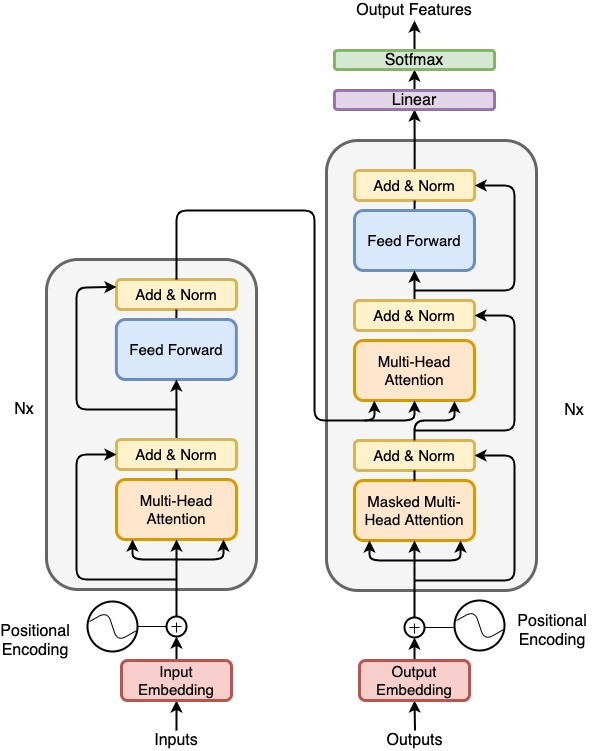
\includegraphics[width=0.6\linewidth]{figs/ch3/transformer_architecture.jpg}
    \caption{This is a reproduction of the graphic presented by~\cite{vaswani2017attention}. The encoder uses self-attention to produce encoding outputs which are fed to the decoder. The decoder uses these encoding outputs and the outputs from its autoregressive self-attention layer to generate the final output text. The graphic shows a single Transformer layer. An actual Transformer model will stack $N$ layers before calculating the output probabilities. }
    \label{fig:transformer_architecture}
\end{figure}

As discussed, the attention mechanism can better model longer-term memory than an RNN hidden state. Attention also allows for better parallelization in training than does the RNN hidden state. Better parallelization implies faster training and more efficient use of compute resources, which creates the capability for bigger models and larger datasets. Due to these reasons, among others, the Transformer has achieved impressive state-of-the-art results over RNN-based models. 

\subsection{Transformer Adaptations: BERT and GPT}
The original Transformer was built with machine translation in mind, but several other NLP tasks could benefit from using an attention-only architecture. Some of these tasks include standard text classification, textual entailment, sentiment analysis, and question answering. A recent trend in NLP research is the pre-training of large models on a single task, which creates generic language data representations fed into models trained for a specific task~\cite{peters2018deep}. BERT is such a model but uses a Transformer architecture for pre-training as opposed to an RNN. BERT is an encoder-only Transformer that significantly increases the original model's parameters and size and is trained on a massive dataset~\cite{devlin2018bert}. The pre-trained representations from BERT are then used with much simpler models trained on specific tasks. This approach led to a significant improvement in the state-of-the-art for general language understanding benchmarks.  

The Generative Pre-Trained Transformer (GPT) is similar to BERT, utilizing only the decoder from the original Transformer instead of the encoder~\cite{radford2019language}\footnote{The model we cite here is the second version of the GPT architecture and is canonically known as GPT-2. A third iteration of GPT, GPT-3, has since been introduced~\cite{brown2020language}. All GPT models use the same model architecture but increase the size of the model and scale of training data at each successive version. We use GPT to refer to all models which use this architecture.}. Like BERT, it is trained on massive amounts of data, is significantly large than the original Transformer, and is used to pre-train a generic language representation that is fed into other models trained for specific tasks. Because GPT is a large Transformer decoder-only language model trained on an immense data corpus, it is capable of writing novel text of surprising quality%
\footnote{Samples of text written by GPT can be found \href{https://openai.com/blog/better-language-models/}{online}}. 

The original Transformer, BERT, and GPT have all significantly improved state-of-the-art for many different tasks NLP. How effective attention-only Transformer models are in other types of sequence data modeling is still an open research question. As we will see in chapter \ref{ch:ch4}, there are already promising results inside the music domain, and even in other fields such as image processing~\cite{dosovitskiy2020image}. 


 